\documentclass{ltjsarticle} %lualatex cs_jikken.texで作成
\usepackage{mdframed}
\usepackage{graphicx}
\usepackage{float}
\usepackage{array}
\usepackage{tikz}
\usepackage{circuitikz}
\usepackage{pgfplots}
\usetikzlibrary{automata, positioning, arrows}
\begin{document}

\thispagestyle{empty}
\begin{flushright}
{\large 実施日 2024年10月19日, 27日{\hspace{5cm}}} 
\end{flushright}

\vspace*{\fill}
\centering
{\Huge\bf コンピュータ科学実験b}
\vspace*{1cm}

{\huge\bf ハードウェア 調査課題}
\vspace*{\fill}

\vspace*{\fill}

\vspace*{\fill}

\begin{flushright}
{\large 学生番号: 102210017} \\ % 5cmの空白を作り、アンダーラインを引く
{\large 氏名: 安藤駿} \\
\end{flushright}

\clearpage

\addtocounter{page}{-1}
\raggedright
\setlength{\parindent}{1em}

\section{はじめに}
これまで様々なモノは個別に役割を果たしていたが, モノにセンサやアクチュエータを搭載し, インターネ
ットに接続可能とすることで, 現実世界の様々な情報収集, モノの遠隔制御, モノ同⼠の相互作⽤が可能とな
る. この考え⽅がIoT(Internet of Things)である. Raspberry Piを⽤いてIoTのデバイス管理を
体験, 学習する. Raspberry Piを⽤いたLED, スイッチ, ステッピングモータの制御を⾏う.


\section{調査課題1(2-2)}

\subsection{チャタリングとは}
チャタリングとは, リレー、スイッチがオンする際に機械的な振動によって短い周期のオン・オフを繰り返すことである. 
スイッチをオンにすると, 接点でスイッチが跳ね返り, 弾性振動により接点とくっついたり離れたりを繰り返す.
これにより, スイッチをオンしてからある間, 負荷にHi-Loのパルス波形が印加されてしまい, スイッチを何度も押したような挙動をしてしまう. 

\subsection{ハードウェア的⽅法による対策}
RCフィルタを用いてチャタリング波形の除去を行う方法がある. これにより, Hi-Loのパルスをなだらかにすることができる. 
しかし, 出力波形が鈍ることと, 出力ラインに抵抗が入るので, 負荷のインピーダンスが低いと電圧降下が発生するというデメリットがある. 


\subsection{ソフトウェア的⽅法による対策}
マイコンで信号を処理する場合は, ソフト処理でフィルタをすることができる. 
マイコンに入力された信号を一定間隔で読み取り, 規定回数連続でHi判定してはじめてHiレベルが入力されたと判定する. 
これにより, チャタリングを防ぐことができる. 

(analogista, 2021)



\section{調査課題2(2-2)}

\subsection{プルアップ及びプルダウンの使用}
プルアップは, 入力ピンがデバイスに接続されていないときに, ピンの状態を安定させるためにHIGHに保つ. 
そして, スイッチが押されたときLOWになる.  
それに対し, プルダウンは, 入力ピンがデバイスに接続されていないときにLOWに保ち, 
スイッチが押されたときHIGHになる. 

つまり, スイッチが押されていないときにピンをHIGHに保ちたい場合にプルアップが使われ, 
LOWに保ちたい場合に, プルダウンが使われる. 


\subsection{プルアップ及びプルダウンの電⼦回路上での実装}
プルアップは, Vcc(3.3Vや5V), 抵抗, 入力ピン(GPIOなど), スイッチ, GNDを図\ref{fig:pullup}のように配置し, 
スイッチが押されていないときはHIGHに保たれている. 
それに対し, プルダウンは, Vcc(3.3Vや5V), 抵抗, 入力ピン(GPIOなど), スイッチ, GNDを図\ref{fig:pulldown}のように配置し, 
スイッチが押されていないときはLOWに保たれている. 

(voltechno, 2019)

\begin{figure}[H]
  \centering  % 全体を中央揃え
  \begin{minipage}{0.45\textwidth}  % 左側の図 (プルアップ回路)
    \begin{center}
      \begin{circuitikz}
        \draw
        % Vcc to Resistor
        (2,2) to[V, l_=$V_{cc}\ (3.3V)$] (4,2)
        % Resistor to GPIO pin
        (4,2) to[R, l_=$10k\Omega$] (6,2)
        (6,2) to[short] (8,2)
        (8,2) node[above]{GPIO pin}
        % GPIO pin to switch
        (6,2) to[switch] (6,0)
        % Switch to GND
        (6,0) to[short] (6,-1)
        (6,-1) node[ground] {};
      \end{circuitikz}
    \end{center}
    \caption{プルアップの実装}
    \label{fig:pullup}
  \end{minipage}
  \hfill  % 図の間にスペースを入れる
  \begin{minipage}{0.45\textwidth}  % 右側の図 (プルダウン回路)
    \begin{center}
      \begin{circuitikz}
        \draw
        % Vcc to switch
        (2,2) to[V, l_=$V_{cc}\ (3.3V)$] (4,2)
        % Switch to Resistor
        (4,2) to[switch] (6,2)
        % Resistor to GPIO pin
        (6,2) to[R, l_=$10k\Omega$] (6,0)
        % GPIO pin
        (6,2) to[short] (8,2)
        (8,2) node[above]{GPIO pin}
        % Resistor to GND
        (6,0) to[short] (6,-1)
        (6,-1) node[ground] {};
      \end{circuitikz}
    \end{center}
    \caption{プルダウンの実装}
    \label{fig:pulldown}
  \end{minipage}
\end{figure}


\section{調査課題3(2-5)}

\subsection{ステッピングモータとは}
ステッピングモータとは制御モータの一種で, 電流を流す相を切り替えることで一定の角度ずつ動いて回転する.
パルスモータ,ステップ,ステッパモータなどとも呼ばれることがある. (techcompass, 2021)

\subsection{ステッピングモータのユニポーラ駆動⽅式}
ステッピングモータは, 固定⼦の励磁する相(SW1 から SW4の各コイル)を, あるシーケンスに従って順番に切
り換えて回転する. ここでは, 3つのユニポーラ駆動⽅式について調べた. 

\subsubsection{1 相励磁⽅式}
1 相励磁⽅式は, 常に固定⼦の1相コイル(巻線)だけを励磁(通電)し, 相を順番に切り換えて回転磁界を作り, 回転⼦を
回転する⽅式である. SW1 から SW4の各コイルは, 表\ref{tab:motor1}に示すように変化する. 

\begin{table}[H] % ここで[h]は表の位置をこの場所にすることを指定します
  \centering % 表を中央に配置
  \caption{1 相励磁⽅式の各相の入力状態}
  \begin{tabular}{|c|c|c|c|c|} 
  \hline % 上の横線
  SW / step & 1 & 2 & 3 & 4 \\ \hline % 行の内容と行間の横線
  SW1 & 1 & 0 & 0 & 0 \\ \hline
  SW2 & 0 & 1 & 0 & 0 \\ \hline
  SW3 & 0 & 0 & 1 & 0 \\ \hline
  SW4 & 0 & 0 & 0 & 1 \\ \hline

  \end{tabular}
  \label{tab:motor1} % 表を参照するためのラベル
\end{table}


\subsubsection{2 相励磁⽅式}
2 相励磁⽅式は, 常に固定⼦の2相コイル(巻線)を励磁(通電)し, 相を順番に切り換えて回転磁界を作り, 回転⼦を
回転する⽅式である. SW1 から SW4の各コイルは, 表\ref{tab:motor2}に示すように変化する. 
常に⼆つの相が励磁されるので, 1相励磁⽅式に比べ, 起動トルクが与えられ乱調が⽣じにくい.
しかし,  1 相励磁に⽐べて2倍の電流容量が必要である.  

\begin{table}[H] % ここで[h]は表の位置をこの場所にすることを指定します
  \centering % 表を中央に配置
  \caption{2 相励磁⽅式の各相の入力状態}
  \begin{tabular}{|c|c|c|c|c|} 
  \hline % 上の横線
  SW / step & 1 & 2 & 3 & 4 \\ \hline % 行の内容と行間の横線
  SW1 & 1 & 1 & 0 & 0 \\ \hline
  SW2 & 0 & 1 & 1 & 0 \\ \hline
  SW3 & 0 & 0 & 1 & 1 \\ \hline
  SW4 & 1 & 0 & 0 & 1 \\ \hline

  \end{tabular}
  \label{tab:motor2} % 表を参照するためのラベル
\end{table}


\subsubsection{1-2 相励磁⽅式}
1-2 相励磁⽅式は, 1 相励磁⽅式と2相励磁⽅式とを交互に⾏うことで回転磁界を作り, 回転⼦を
回転させる⽅式である. SW1 から SW4の各コイルは, 表\ref{tab:motor1-2}に示すように変化する. 
ステップ⾓はハーフ・ステップになるので, 回転速度は, 1相励磁⽅式や2相励磁⽅式の半分となる. 

\begin{table}[H] % ここで[h]は表の位置をこの場所にすることを指定します
  \centering % 表を中央に配置
  \caption{1-2 相励磁⽅式の各相の入力状態}
  \begin{tabular}{|c|c|c|c|c|c|c|c|c|} 
  \hline % 上の横線
  SW / step & 1 & 2 & 3 & 4 & 5 & 6 & 7 & 8\\ \hline % 行の内容と行間の横線
  SW1 & 1 & 1 & 1 & 0 & 0 & 0 & 0 & 0\\ \hline
  SW2 & 0 & 0 & 1 & 1 & 1 & 0 & 0 & 0\\ \hline
  SW3 & 0 & 0 & 0 & 0 & 1 & 1 & 1 & 0\\ \hline
  SW4 & 1 & 0 & 0 & 0 & 0 & 0 & 1 & 1\\ \hline

  \end{tabular}
  \label{tab:motor1-2} % 表を参照するためのラベル
\end{table}

\section{調査課題4(2-5)}

\subsection{台形速度制御とは}
台形速度制御とは, モーターやロボットなどの機械を制御する際に, 目標速度に到達するまでの
速度の変化を図\ref{fig:graph1}で示すように, 台形のような形に設定する制御方法である. 
この手法は, 機械を滑らかに加速, 減速させるために用いられる. 
加速区間, 定速区間, 減速区間の3つのフェーズに分けらる.  
加速区間は, 一定の加速度で速度を上昇させる区間であり, 設定された最大速度に到達すると終了する. 
定速区間は, 速度が最大に達した後, この速度を一定に保ちながら機械を動作させる区間である. 
減速区間は, 停止するために一定の加速度で速度を落とす区間である. 


(Tajima, 2019)

\begin{figure}[H]
  \centering
  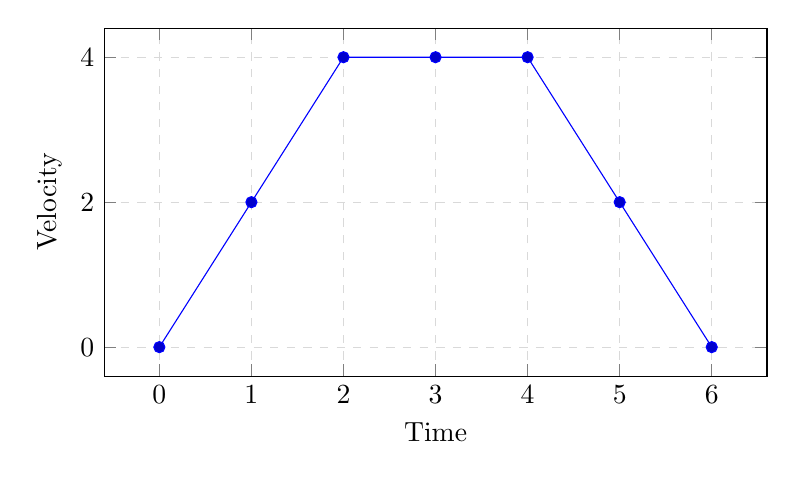
\begin{tikzpicture}
      \begin{axis}[
          xlabel={Time},
          ylabel={Velocity},
          grid=both,
          width=10cm,
          height=6cm,
          grid style={dashed, gray!30},
          ]
          % 折れ線グラフのデータ
          \addplot coordinates {
              (0,0) (1,2) (2,4) (3,4) (4,4) (5,2) (6,0)
          };
      \end{axis}
  \end{tikzpicture}
  \caption{台形加速}
  \label{fig:graph1}
\end{figure}


\subsection{ステッピングモータの台形速度制御}
課題2-4で作成したステッピングモータの制御をするコードのtime.sleepの値を変化させることで
台形加速をするコードdaikei.pyを作成した. これを図\ref{fig:daikeipy}に示す. 
TIME SLEEP INITIALは初期のtime.sleepの停止時間であり, 減速区間でこの値まで停止時間を長くしていく. 
TIME SLEEP FASTESTは定速区間のtime.sleepの停止時間であり, 加速区間でこの値まで停止時間を短くしていく. 
ACCELERATION STEPSは, 加速, 減速に用いるステップ数である. 
TOTAL STEPSは, 全体のステップ数であり, TOTAL STEPS - 2 * ACCELERATION STEPS の値が定速区間のステップ数である. 
current sleepはステップごとの停止時間を示している. 

加速区間で, (TIME SLEEP INITIAL - TIME SLEEP FASTEST) / ACCELERATION STEPSの値だけ, 停止時間を短くする. 
その後停止時間がTIME SLEEP FASTESTと同じになったら, 定速区間へ移る. 
減速区間でも同様に停止時間を長くし, 停止する. 

このようにsleep timeで停止させる時間を制御することで台形速度制御を実装した. 
しかし, 停止時間を調整するだけでステッピングモータの速度を完全に制御できるかどうか分からない.  
特にモータカーとして走らせる際に, 荷重によりトルク不足などの問題が起き完全な台形加速にならないかもしれない.  
そのため, 実際に稼働させてみることが必要だと考えた. 


\begin{mdframed}
  \begin{verbatim}
    from gpiozero import OutputDevice
    import time
    
    # ステッピングモータ接続GPIO端⼦番号
    OUTPUT_PIN1_1 = 6
    OUTPUT_PIN1_2 = 13
    OUTPUT_PIN1_3 = 19
    OUTPUT_PIN1_4 = 26
    
    # 初期のモータ回転間隔
    TIME_SLEEP_INITIAL = 0.01
    
    # 定速運転時のモータ回転間隔
    TIME_SLEEP_FASTEST = 0.002
    
    # 加速・減速に使うステップ数
    ACCELERATION_STEPS = 100
    
    # 全体の運転ステップ数
    TOTAL_STEPS = 1000
    
    # モータ⽤の出⼒端⼦を⽣成する
    motor_pins = [
        OutputDevice(OUTPUT_PIN1_1),
        OutputDevice(OUTPUT_PIN1_2),
        OutputDevice(OUTPUT_PIN1_3),
        OutputDevice(OUTPUT_PIN1_4),
    ]
    
    # 指定した1相のみを励磁する関数
    def out_motor_pin(pin_num):
        for i in range(0, 4):
            if i == pin_num:
                motor_pins[i].on()
            else:
                motor_pins[i].off()
    
    
    #台形加速開始
    
    #最初のtime.sleepの時間
    current_sleep = TIME_SLEEP_INITIAL
    
    i = 0
    # 加速区間
    for step in range(ACCELERATION_STEPS):
        out_motor_pin(i)
        i = (i + 1) % 4
        time.sleep(current_sleep)
        
        # 加速:ステップごとに待機時間を短くしていく
        current_sleep -= (TIME_SLEEP_INITIAL - TIME_SLEEP_FASTEST) / ACCELERATION_STEPS
        if current_sleep < TIME_SLEEP_FASTEST:
            current_sleep = TIME_SLEEP_FASTEST
    
    # 定速区間
    for step in range(TOTAL_STEPS - 2 * ACCELERATION_STEPS):
        out_motor_pin(i)
        i = (i + 1) % 4
        time.sleep(current_sleep)
    
    # 減速区間
    for step in range(ACCELERATION_STEPS):
        out_motor_pin(i)
        i = (i + 1) % 4
        time.sleep(current_sleep)
        
        # 減速:ステップごとに待機時間を長くしていく
        current_sleep += (TIME_SLEEP_INITIAL - TIME_SLEEP_FASTEST) / ACCELERATION_STEPS
        if current_sleep > TIME_SLEEP_INITIAL:
            current_sleep = TIME_SLEEP_INITIAL	
  \end{verbatim}
\end{mdframed}
\begin{figure}[H]
  \caption{daikei.py}
  \label{fig:daikeipy}
\end{figure}


\section{調査課題5}

\subsection{I2Cとは}
I2C(Inter-Integrated Circuit)とは, Philips Semiconductors社(現在のNXP Semiconductors社)が開発した通信規格である. 
IC間の通信を担い, マイコンとその周辺機器(EEPROMなど)の通信でよく使われる. 

\subsection{SDAとSCL}
I2Cでは, SDAとSCLの2本の信号線を用いて通信を行う. 
SDAはSerial Dataの略で, データ用の信号線であり, SCLはSerial Clockの略で, クロック用の信号線である. 
それぞれの信号線にはプルアップ抵抗が接続される. 

\subsection{マスタとスレーブ}
I2Cでは, デバイスはその役割によってマスタとスレーブに分けらる. 
マスタは通信の開始, クロック信号の生成, 通信の終了を行う. 
マスタはスレーブが持つスレーブアドレスを指定することで特定のスレーブと通信する. 
図\ref{fig:fig1}のように, 1つのマスタと複数のスレーブをSDAとSCLに接続する. 

(ensatellite, 2021)

\begin{figure}[H] % 画像を挿入する環境を開始
  \centering
  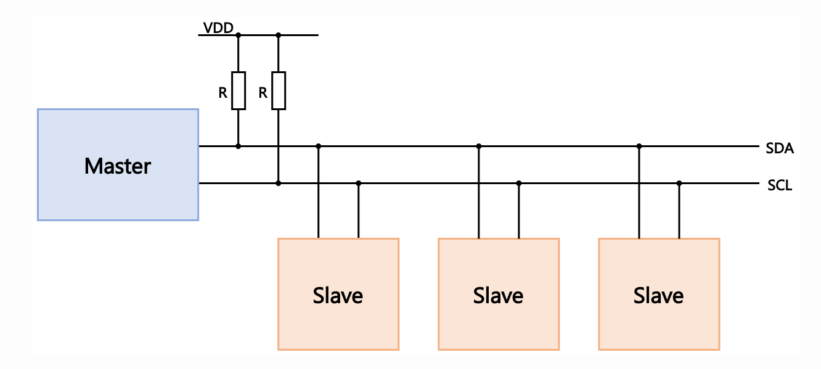
\includegraphics[width=0.8\textwidth]{fig1.png} % 画像を挿入、幅をページ幅に合わせる
  \caption{SDAとSCLの接続} % キャプションを追加
  \label{fig:fig1} % ラベルを追加
\end{figure}


\section{調査課題6}

\subsection{AD変換とは}
A/D変換(Analog-to-Digital Conversion)とは, アナログ信号をデジタル信号に変換するプロセスのことである. 
標本化, 量子化, 符号化の順にデジタル信号に変換していく. 
標本化とは, 連続なアナログ信号の振幅値を離散的な周期で切り出すことである. 
量子化とは, 離散的な周期で切り出された振幅値を、離散的な振幅値に近似することである. 
符号化とは, 離散的な振幅値を"0"と"1"の2値で表す符号に変換することである. 
このような手順で, 連続値であるアナログ信号の各ポイントをサンプリングし, それを離散値であるデジタル値として表現していく. 

A/D変換は, 音声データのデジタル化や温度, 圧力, 光の強さなどのセンサー値のデジタル化, 医療機器や測定機器でのデータ処理
などに使われている. 

\subsection{D/A変換とは}
D/A変換(Digital-to-Analog Conversion)とは, デジタル信号をアナログ信号に変換するプロセスのことである. 
電圧または電流に変換, 平滑化の順にアナログ信号に変換していく. 
電圧または電流に変換では, 入力されたデジタル値を基に、コンバータが対応するアナログ電圧または電流を出力する. 
平滑化では, デジタル値の変換は階段状になるため、スムーズな連続信号を得るために低パスフィルタを使用する. 

D/A変換は, 音楽再生, ビデオ再生などで使用されている. 

(pabasic, 2016)


\begin{thebibliography}{99} % 最大ラベル幅を99に設定
    
    \bibitem{lamport1994latex}
    PassMark: 
    \emph{チャタリングとは?原因と対策方法について}. \\
    \verb|https://analogista.jp/chattering/|  2021.
  
    \bibitem{lamport1994latex}
    PassMark: 
    \emph{プルアップ抵抗・プルダウン抵抗とは?電子回路に必須の考え方}. \\
    \verb|https://voltechno.com/blog/pullup-pulldown/|  2019.
  
    \bibitem{lamport1994latex}
    PassMark: 
    \emph{ステッピングモータとは?}. \\
    \verb|https://techcompass.sanyodenki.com/jp/training/servo/motor_tips/001/index.html|  2021.

    \bibitem{lamport1994latex}
    PassMark: 
    \emph{台形速度の軌跡生成をしてロボットを制御する方法}. \\
    \verb|https://tajimarobotics.com/acceleration-limited-feed-profile-2/|  2019.

    \bibitem{lamport1994latex}
    PassMark: 
    \emph{I2Cの概要と仕組み}. \\
    \verb|https://ensatellite.com/ja/i2c/|  2021.

    \bibitem{lamport1994latex}
    PassMark: 
    \emph{AD変換とDA変換の基本: デジタル機器の心臓部}. \\
    \verb|https://pabasic.com/100_engineer/105_digital/ad-da/|  2016.
  
\end{thebibliography}
  
  
\end{document}